% -*- coding: utf-8 -*-
\documentclass{article}
\usepackage{polski}
%\usepackage[T1]{fontenc}
%\usepackage[utf8]{inputenc}
\usepackage{xltxtra}
\usepackage{listings}
\usepackage{fullpage}
\usepackage{graphicx}
\usepackage{color}
\usepackage{amsmath}
\usepackage{amsthm}
\usepackage{indentfirst}
\usepackage{hyperref}
\newtheorem{twi}{Twierdzenie}
\author{Karol Piotrowski, Krzysztof Pater}
\title{Algorytmy i Struktury Danych, projekt\\ Algorytm Dinica znajdowania największego przepływu}
\begin{document}
\maketitle
\section{Wstęp}
Niedługo minie 60 lat, od kiedy Ford i Fulkerson dowiedli w pracy [1] twierdzenia:
\begin{twi} Niech $S=(G,c)$ będzie siecią przepływową. Wówczas jeśli $A, V\setminus A$ jest przekrojem minimalnym ze względu na wartość $c(A)=\sum_{u \in A. v\notin A} c(u,v)$ to dla dowolnego przepływu $f$ w sieci $S$ zachodzi nierówność $c(A) \leq |f|$, a ponadto istnieje przepływ maksymalny, dla którego zachodzi równość.
  \end{twi}
Nietrywialną częścią było wykazanie, że maksymalny przepływ rzeczywiście istnieje (minimalny przekrój nie trudno sobie wyobrazić biorąc pod uwagę fakt, że jest skończona liczba zbiorów wierzchołków), zaś zaproponowany przez Forda i Fulkersona algorytm miał złożoność czasową $O(|V|\cdot \max_{e\in E} c(E))$, zatem poza szczególnymi przypadkami niewielkie zastosowanie praktyczne. Od tego czasu powstało wiele algorytmów zarówno teoretycznych jak i praktycznych, a w 2013 roku świat obiegła informacja o prawie liniowym aproksymacyjnym algorytmie znajdowania maksymalnego przepływu (patrz praca [2]). Celem tego projektu będzie zbadanie empiryczne jednego z podstawowych algorytmów, opracowanego przez Dinica. Będziemy zajmować się wersją klasyczną, działającą w czasie $O(|V|^2|E|)$, gdyż wersja ta jest prostsza i bardziej czytelna w implementacji niż np. modyfikacja znana jako algorytm trzech Hindusów (MKM, patrz [3]), która działa w czasie $O(|V|^3)$, a więc powinna sprawdzać się lepiej dla sieci wypełnionych krawędziami (takich, że $|E| = \Omega(|V|^2)$). 

\section{Opis i analiza algorytmu}
  Omówimy krótko klasyczną wersję algorytmu Dinica dla sieci nieskierowanych. Implementacji dokonano ze względów dydaktycznych w języku Python, z zastosowaniem wbudowanych dynamicznych struktur danych (\texttt{list()} jako tablica, gdyż zgodnie ze standardem języka jest ona realizowana jako tablica dynamiczna z kosztem amortyzowanym zarówno zapisywania, jak i odczytywania $O(1)$ oraz \texttt{collections.deque} jako stos/kolejka, gdyż jest to w rzeczywistości lista dwukierunkowa). Do zapisu tablicy list sąsiedztwa w grafie użyto \texttt{list()} dla prostoty zapisu (i tak iterujemy prawie zawsze od początku listy i dopisujemy na ,,właściwym" końcu). 
  
W dowodzie poprawności działania algorytmu Dinica wykorzystamy łatwą część twierdzenia Forda i Fulkersona, tj.
\begin{twi} Niech $(G,c)$ będzie siecią przepływową, $f$ przepływem na $(G,c)$. Wówczas następujące warunki są równoważne:
  \begin{enumerate}
   \item $f$ jest przepływem maksymalnym, 
   \item w $(G,c)$ nie istnieje ścieżka powiększająca,
   \item $|f| = c(A, V\setminus A)$ dla pewnego przekroju $A, V\setminus A$.
  \end{enumerate}
\end{twi}
Prosty dowód można znaleźć na przykład w podręczniku [4], na podstawie którego zresztą powstała część omówienia algorytmu.

Algorytm Dinica jest jednym z algorytmów wykorzystujących tzw. przepływy blokujące. \emph{Przepływ blokujący} to taki, w którym każda ścieżka od źródła do ujścia zawiera krawędź nasyconą (taką, że $f(u,v) = c(u,v)$).

Idea jest następująca: tworzymy \emph{pomocniczą sieć acykliczną}, zawierającą informację, o ile zadany w sieci przepływ można powiększyć. Ściśle rzecz biorąc, konstruujemy ją w następujący sposób:
\begin{itemize}
\item Ustalamy tablicę $\mathtt{ODL[v]}$ odległości wierzchołków od źródła, kładąc $\mathtt{ODL[s]}=0, \mathtt{ODL[v]}=\inf$ dla $v\neq s$. W trakcie odwiedzania sieci (BFSem) wyznaczamy ścieżki $s\to t$, przy czym po ustaleniu się odległości $\mathtt{ODL[t]}$ nie odwiedzamy wierzchołków dalszych. 
\item Przeszukujemy wgłąb tylko krawędzie \emph{użyteczne}, takie, wzdłuż których można powiększyć przepływ, tj. albo $\mathtt{ODL[u]} +1 = \mathtt{ODL[v]}$ (kierujemy się w stronę celu) oraz $f[u,v] < c[u, v]$ (krawędź nie jest nasycona), albo krawędź prowadzi w stronę od celu do źródła i ma niezerowy przepływ (w takim wypadku zastępujemy ją odpowiednią krawędzią w stronę przeciwną). W sytuacji, gdy istnieją krawędzie użyteczne zarówno $u\to v$, jak i $v\to u$, również bierzemy to pod uwagę.
\item Użyteczne krawędzie zapisujemy w sieci $G_f$ przypisując im przepustowości:
\begin{itemize}
  \item $c_f (u,v) = c(u,v) - f(u,v)$ dla krawędzi użytecznych w stronę od źródła do celu, 
  \item $c_f (u,v) = f(v,u)$ dla krawędzi użytecznych od celu do źródła, 
  \item $c_f (u,v) = c(u,v) - f(u,v) + f(v,u)$ dla par krawędzi użytecznych $u\to v, v\to u$ (samą krawędź ustalamy w stronę $s\to t$).
\end{itemize}
\end{itemize}
Postępując w tę stronę dostajemy \emph{pomocniczą sieć acykliczną}. Acykliczność sieci jest oczywista, w trakcie BFS nie da się odwiedzić tego samego wierzchołka dwukrotnie. 

Działanie algorytmu jest jasne ze względu na fakt, że algorytm nie opuszcza pętli dopóki istnieje chociaż jedna ścieżka od źródła do ujścia na której istnieje krawędź nienasycona. 
\section{Empiryczne testy stworzonej implementacji}
W wykonanej aplikacji ,,Algorytm Dinica" umieszczono możliwość wykonywania testów czasu działania algorytmu i generowania na ich podstawie wykresów. Ze względu na dużą złożoność obliczeniową i wymagania pamięciowe (ze względu na przechowywanie tablicy przepustowości potrzeba $O(|V|^2)$ pamięci) testy przeprowadzono dla zakresu do około 100 wierzchołków grafu. W pierwszej kolejności zbadano średni czas wykonania algorytmu dla $|V|=30$ i zmieniającej się liczby krawędzi:
\begin{center}
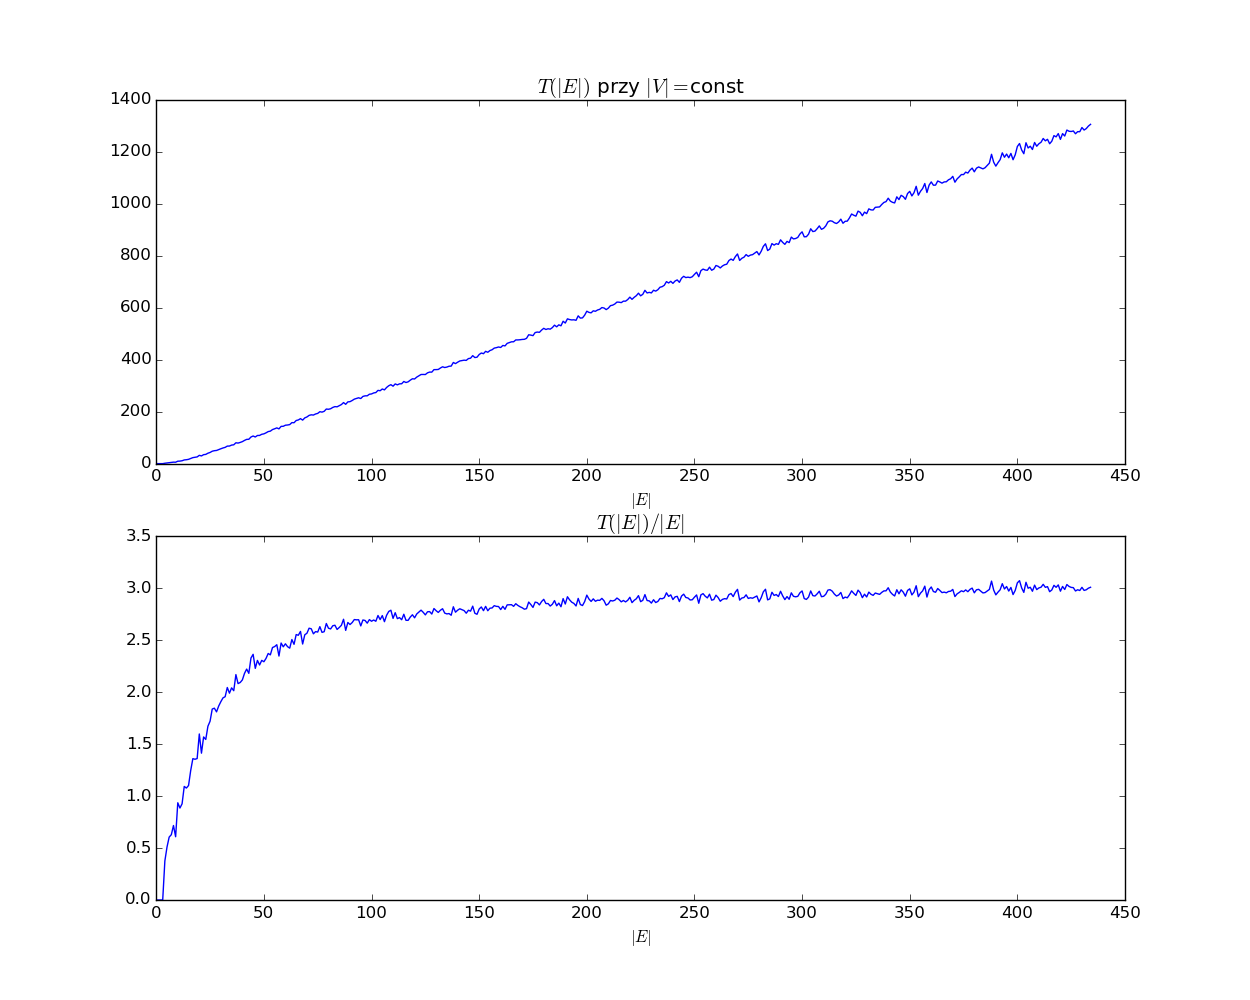
\includegraphics[scale=0.55]{constv.png}
\end{center}
Czas wykonania przedstawiono w jednostkach umownych--$T(|E|) = t(|E|)/t(3)$, gdzie $t$ jest średnim czasem pracy algorytmu w sekundach. Przedstawione dane doświadczalne ilustrują fakt, że przy ustalonym $|V|$ czas działania algorytmu jest liniowy ze względu na $|E|$ ($T(|E|)/|E|$ jest praktycznie stałe dla dużych $|E|$).

W następnej kolejności zbadano (i wyrażono w jednostkach umownych podobnie jak w poprzednim przypadku) czas działania algorytmu dla sieci o małej liczbie krawędzi ($|E| = O(|V|)$) dla $|V|\leq 100$, dane umieszczono na wykresie: 
\begin{center}
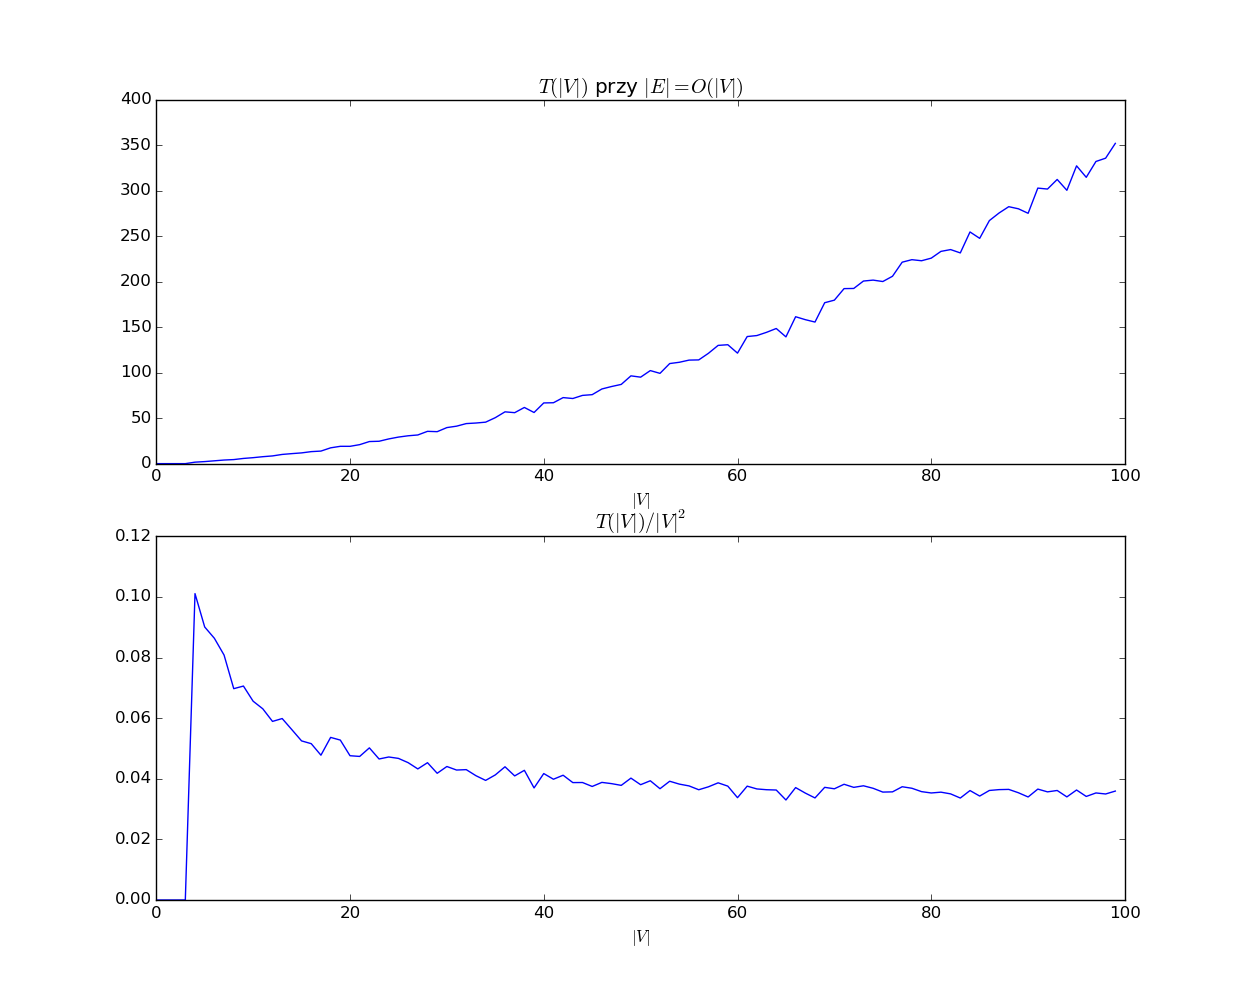
\includegraphics[scale=0.55]{malee.png}
\end{center}
Jak widać, $T(|V|)/|V|^2$ jest stałe dla szerokiego zakresu $|V|$, co ilustruje kwadratową \emph{średnią} złożoność algorytmu dla $|E|=O(|V|)$. Oszacowanie pesymistyczne to $O(|V|^3)$, jednak przy losowym generowaniu sieci bardzo często algorytm zatrzymuje się szybciej, gdyż w ogóle nie ma drogi od źródła do ujścia. 



\end{document}
